\documentclass[11pt]{amsart}
\usepackage{amsmath,amssymb,amsthm}
\usepackage{graphicx}
\usepackage{hyperref}
\renewcommand{\sfdefault}{\rmdefault}
\hypersetup{colorlinks=true,linkcolor=blue,citecolor=blue,urlcolor=blue}

\newtheorem{theorem}{Theorem}[section]
\newtheorem{proposition}[theorem]{Proposition}
\newtheorem{lemma}[theorem]{Lemma}
\theoremstyle{remark}
\newtheorem{remark}[theorem]{Remark}
\DeclareMathOperator{\Law}{Law}
\DeclareMathOperator{\RePart}{Re}
\newcommand{\Torus}{\mathbb{T}^{2}_{L}}
\newcommand{\Hthree}{H^{-3}_{\mathrm{Fourier}}}
\newcommand{\Htwo}{H^{-2}_{\mathrm{Fourier}}}
\newcommand{\Pmeas}{\mathcal{P}}

\title[Fixed-volume weak convergence]{Whole-Sequence Weak Convergence of Fixed-Volume Lattice Free Fields on a Periodic $H^{-3}$ Carrier}
% AUTHOR_INPUT_NEEDED: supply author names and affiliations before submission.
\date{}

\begin{document}
\begin{abstract}
We prove whole-sequence weak convergence of the concrete fixed-volume periodic lattice free-field laws on a weighted Fourier carrier of negative Sobolev order three. For a positive period and positive mass, the nth law is the pushforward of a finite-dimensional Gaussian measure with lattice size equal to n plus one and spacing equal to the period divided by that size. A uniform negative-order-two energy moment yields tightness in the negative-order-three carrier; fixed-volume covariance convergence identifies every finite weighted Fourier marginal with the periodic massive-resolvent Gaussian law. Separability, Prokhorov extraction, Borel generation by finite-coordinate cylinders, and measure uniqueness identify every subsequential limit and imply convergence of the entire sequence to an actual Borel probability measure. The proof is formalized in Lean in the project's dedicated Pphi2 clean package. We distinguish this finite-source sequence from a separate physical-lattice total-carrier pushforward that still requires a named lift input.
\end{abstract}
\maketitle

\section{The question and the proof strategy}

A finite-dimensional Gaussian law at each mesh size does not by itself produce a probability law on an infinite-dimensional function space. Nor does convergence of every fixed finite collection of Fourier coefficients, on its own, imply weak convergence of the full laws. The fixed-volume limit therefore has two logically separate obligations: compactness of the sequence as measures on one specified carrier, and identification of every possible limit on a class of sets rich enough to determine a Borel measure.

We address the implication
\[
  \mu_n \Longrightarrow \mu_{\mathrm{free}}
\]
for a particular two-dimensional periodic lattice sequence, with every object in the statement tied to the formal source. The source fixes $N_n=n+1$ sites per coordinate and spacing $a_n=L/N_n$, so the physical period is exactly $L$ at every stage. Each $\mu_n$ is the pushforward of a finite-source Gaussian configuration law by the explicit weighted Fourier lift into a complete weighted $\ell^2$ space.

The proof has a compactness half and an identification half. A uniform second-moment estimate in the weaker $H^{-2}$ weight, together with compact inclusion into the $H^{-3}$ carrier, gives tightness. Prokhorov's theorem then supplies limits along further subsequences. In parallel, the finite-dimensional covariance matrices converge to those of the periodic massive resolvent, so every finite weighted Fourier cylinder of every extracted limit has the same Gaussian law. Since the carrier is separable and its finite-coordinate cylinders generate its Borel sigma-algebra, these marginals determine the limit measure. The subsequence criterion then yields convergence of the whole sequence. Figure~\ref{fig:proof-spine} summarizes this dependency chain; it is explanatory, while the Lean declarations in Appendix~\ref{app:formal-evidence} are the formal evidence.

The construction is deliberately not reduced to a compatible family of finite-dimensional distributions. Prokhorov extraction constructs a probability measure on the carrier first; the cylinder argument subsequently identifies it. This ordering is what closes the implication from $\mu_n$ to an actual $\mu_{\mathrm{free}}$.

The background compactness and subsequence principles are standard; see, for example, Billingsley~\cite{billingsley}. Our contribution here is the assembled, source-specific theorem with its concrete sequence, moment estimate, covariance limit, carrier topology, and measure-uniqueness step all connected in the Lean development. We make no priority claim.

\section{Carrier and main theorem}
\label{sec:theorem}

Let $\mathbb{Z}^{2}$ index Fourier modes. Define
\[
 w_3(0)=1,\qquad w_3(k)=|k|^{-6}\quad(k\ne 0).
\]
Set $\Hthree=\ell^2(\mathbb{Z}^{2},\mathbb{C})$ in stored coordinates $x(k)=\sqrt{w_3(k)}c(k)$; equivalently, raw Fourier coefficients $c$ have squared norm $\sum_k w_3(k)|c(k)|^2$. The complex carrier is the weighted completion used in Lean and is not restricted by an additional conjugate-symmetry condition. The finite Fourier coordinate map for a mode list $K=(k_1,\ldots,k_r)$ is
\[
  \mathrm{C}_K(x)=(x(k_1),\ldots,x(k_r))\in\mathbb{C}^{r}.
\]
Each coordinate map is continuous.

For each $n\in\mathbb{N}$ set $N_n=n+1$ and $a_n=L/N_n$. Let $\gamma_n^{L,M}$ denote the finite-dimensional centered Gaussian configuration probability measure with the source's numbered periodic lattice covariance, and let $J_n^{L,M}$ be the explicit finite-source Fourier lift into the weighted coordinates. The sequence studied here is
\[
  \mu_n^{L,M}=(J_n^{L,M})_{\#}\gamma_n^{L,M}
  \in\Pmeas(\Hthree).
\]
In particular, it is a finite-source pushforward, not a law defined from the separate physical-Gaussian total-carrier representative.

For a finite mode list $K$, let $f_{j,0}$ and $f_{j,1}$ be the real cosine and sine test functions specified by the formal development for mode $k_j$. Define the real covariance matrix
\[
  (\Sigma_K)_{(j,s),(\ell,t)}
  =\RePart\,\mathcal{R}_{L,M}(f_{j,s},f_{\ell,t}),
  \qquad s,t\in\{0,1\},
\]
where $\mathcal{R}_{L,M}$ is the physical-volume pairing with the weak solution of the massive periodic equation. Its Fourier mass symbol is
\[
  \lambda_{L,M}(k)=M^2+\left(\frac{2\pi}{L}\right)^2|k|^2.
\]
This definition fixes the physical $L^2$ pairing and avoids an independent Fourier-normalization convention. Let $G_K$ be the centered real Gaussian probability measure on $\mathbb{R}^{2r}$ with covariance $\Sigma_K$, including the possibly degenerate case. Define
\[
  \Psi_K(y)_j=\sqrt{w_3(k_j)}\bigl(y_{j,0}+i y_{j,1}\bigr),
  \qquad y\in\mathbb{R}^{2r}.
\]

\begin{theorem}[Fixed-volume weak limit and Fourier marginals]
\label{thm:main}
For every $L>0$ and $M>0$, there exists a Borel probability measure
$\mu_{\mathrm{free}}^{L,M}\in\Pmeas(\Hthree)$ such that
\[
  \mu_n^{L,M}\Longrightarrow\mu_{\mathrm{free}}^{L,M}
  \quad\text{as }n\to\infty.
\]
Moreover, for every finite mode list $K$,
\[
  (\mathrm{C}_K)_{\#}\mu_{\mathrm{free}}^{L,M}
  =(\Psi_K)_{\#}G_K.
\]
These finite weighted Fourier marginals determine $\mu_{\mathrm{free}}^{L,M}$ uniquely among Borel probability measures on $\Hthree$.
\end{theorem}

Here weak convergence is the probability-measure topology on the Polish carrier, equivalently convergence against bounded continuous real test functions. The assembled theorem and its declaration are documented in Appendix~\ref{app:formal-evidence}.

\section{Uniform moment control and tightness}
\label{sec:tightness}

The H$^{-2}$ weight used for the moment estimate is
\[
 w_2(0)=1,\qquad w_2(k)=|k|^{-4}\quad(k\ne0).
\]
In two dimensions, $\sum_{k\ne0}|k|^{-4}$ is finite. The source proves the explicit fixed-volume trace bound
\begin{align}
 \int_{\Hthree} E_{-2}(x)\,d\mu_n^{L,M}(x)&\le C_{L,M},
 \label{eq:trace-bound}\\
 C_{L,M}&:=M^{-2}L^2\left(1+2\sum_{k\in\mathbb{Z}^2\setminus\{0\}}|k|^{-4}\right)\\
       &<\infty,\qquad n\in\mathbb{N}.
\end{align}
where $E_{-2}$ is the extended H$^{-2}$ energy on the H$^{-3}$ carrier. The zero mode contributes the separate $M^{-2}L^2$ term. This bound is proved for the actual pushforward probability measures $\mu_n^{L,M}$, not just for a formal covariance trace.

For $R>0$, consider the H$^{-2}$ energy sublevel
\[
  K_R=\{x\in\Hthree:E_{-2}(x)\le R^2\}.
\]
The weighted inclusion from H$^{-2}$ to H$^{-3}$ is compact: on nonzero modes the ratio of squared weights is $w_3(k)/w_2(k)=|k|^{-2}$, which tends to zero as $|k|\to\infty$; the zero mode is finite-dimensional. The formal development proves compactness of the relevant closed sublevels in the concrete completion. Measurability of the energy and Markov's inequality applied to \eqref{eq:trace-bound} give
\[
  \sup_n\mu_n^{L,M}(K_R^c)\le \frac{C_{L,M}}{R^2}.
\]
Thus, given any $\varepsilon>0$, a sufficiently large $R$ gives one compact set carrying at least $1-\varepsilon$ of every measure. The family is tight.

The carrier is complete by construction and separable by density of finite-coordinate truncations. It is therefore Polish, so Prokhorov's theorem applies. From every subsequence of $(\mu_n^{L,M})$ one can extract a further subsequence converging weakly to a Borel probability measure on the same carrier~\cite{billingsley}. The extracted measure is not postulated: it is the actual limit delivered by this compactness step.

\section{Finite Fourier convergence and the target law}
\label{sec:marginals}

Fix a finite mode list $K$. The finite-source lift sends its paired cosine and sine evaluations to the weighted complex coordinate vector $\mathrm{C}_K$. Before complexification, these evaluations form a centered finite-dimensional Gaussian vector. Its covariance entries are the corresponding finite-lattice covariance pairings.

For each fixed periodic test function, the finite-volume lattice covariance converges to the physical periodic-resolvent pairing $\mathcal{R}_{L,M}$. At the Fourier level, the limiting denominator at mode $k$ is
\[
  M^2+\left(\frac{2\pi}{L}\right)^2|k|^2,
\]
which is exactly the mass symbol used in the formalized resolvent. The finite-family convergence theorem applies entrywise to the covariance matrix and proves weak convergence of the real Gaussian evaluation law to $G_K$. This argument includes degenerate covariance matrices and does not require a nonsingular density.

The continuous reassembly map $\Psi_K$ multiplies the cosine--sine pair by $\sqrt{w_3(k_j)}$ and forms the complex coefficient. By the continuous mapping theorem, the pushed-forward finite-coordinate law converges to $(\Psi_K)_{\#}G_K$. Since $K$ was arbitrary, this proves the finite-cylinder convergence needed for the infinite-dimensional argument.

No additional universal test-function convergence assumption is inserted at this step: the required cosine/sine family is constructed from the requested mode list, and the covariance limit is proved for that concrete family. The target is specified by the physical resolvent pairing and its Lean-defined mass symbol; no unstated prefactor or Fourier convention is used.

\section{Cylinder uniqueness closes the whole sequence}
\label{sec:identification}

Every weak subsequential limit $\nu$ has the target marginal $(\Psi_K)_{\#}G_K$ for each finite mode list $K$. Indeed, the coordinate maps are continuous, so weak convergence on the carrier implies weak convergence of their pushforwards. The full sequence of pushforward laws already converges to the target by Section~\ref{sec:marginals}; uniqueness of limits in the finite-dimensional probability-measure space identifies the pushforward of $\nu$ with that same target.

It remains to show that these finite marginals determine the carrier law. The coordinate maps generate the cylinder pi-system. Every such cylinder is Borel. Separability of the weighted $\ell^2$ carrier makes it Polish, and the formal development proves that the sigma-algebra generated by finite-coordinate cylinders equals the carrier Borel sigma-algebra. The finite-measure uniqueness theorem therefore implies that any two Borel probability measures with the same finite weighted Fourier marginals coincide.

Choose one Prokhorov limit and call it $\mu_{\mathrm{free}}^{L,M}$. The preceding argument shows that every extracted limit has the same finite marginals as this measure, hence equals it. To see that the original sequence converges, suppose it did not. Then some neighborhood of $\mu_{\mathrm{free}}^{L,M}$ would be missed along a subsequence. Tightness would give a further weakly convergent subsequence; its limit must equal $\mu_{\mathrm{free}}^{L,M}$, contradicting that it stays outside the neighborhood. Thus the entire sequence converges.

This step is stronger than identifying one convergent subsequence. It uses the fact that every subsequence admits a further limit and that the Borel cylinder marginals leave no freedom in that limit. The resulting $\mu_{\mathrm{free}}^{L,M}$ is an actual Borel probability measure, and its construction and uniqueness are both part of Theorem~\ref{thm:main}.

\section{What the theorem does and does not identify}
\label{sec:scope}

The theorem proves weak convergence for the explicit finite-source sequence defined in Section~\ref{sec:theorem}. The limiting Borel probability measure is constructed by tightness and subsequential extraction, then uniquely identified through its finite weighted Fourier marginals. The statement is for a two-dimensional periodic carrier, with fixed period $L>0$ and mass $M>0$.

A separate construction in the Lean package starts from the physical lattice Gaussian measure `physicalGJMeasure` and maps its total representative into the same carrier. That map requires a named `PeriodicHMinusThreeLiftMeasureInput` for measurability and almost-everywhere representative agreement. It is not the source of the sequence in Theorem~\ref{thm:main}, and the theorem does not use or discharge that input. Keeping the two maps distinct avoids treating a conditional physical-lattice bridge as part of an unconditional finite-source theorem.

The result does not assert an interacting-field limit, an Osterwalder--Schrader reconstruction, an infinite-volume limit, a theorem in other dimensions, or an identification with a separately specified distribution-space model. The construction provides a measure through Prokhorov compactness and characterizes it by finite Fourier laws; it does not claim a samplewise Fourier-series representation beyond what those statements entail.

\begin{figure}[tb]
  \centering
  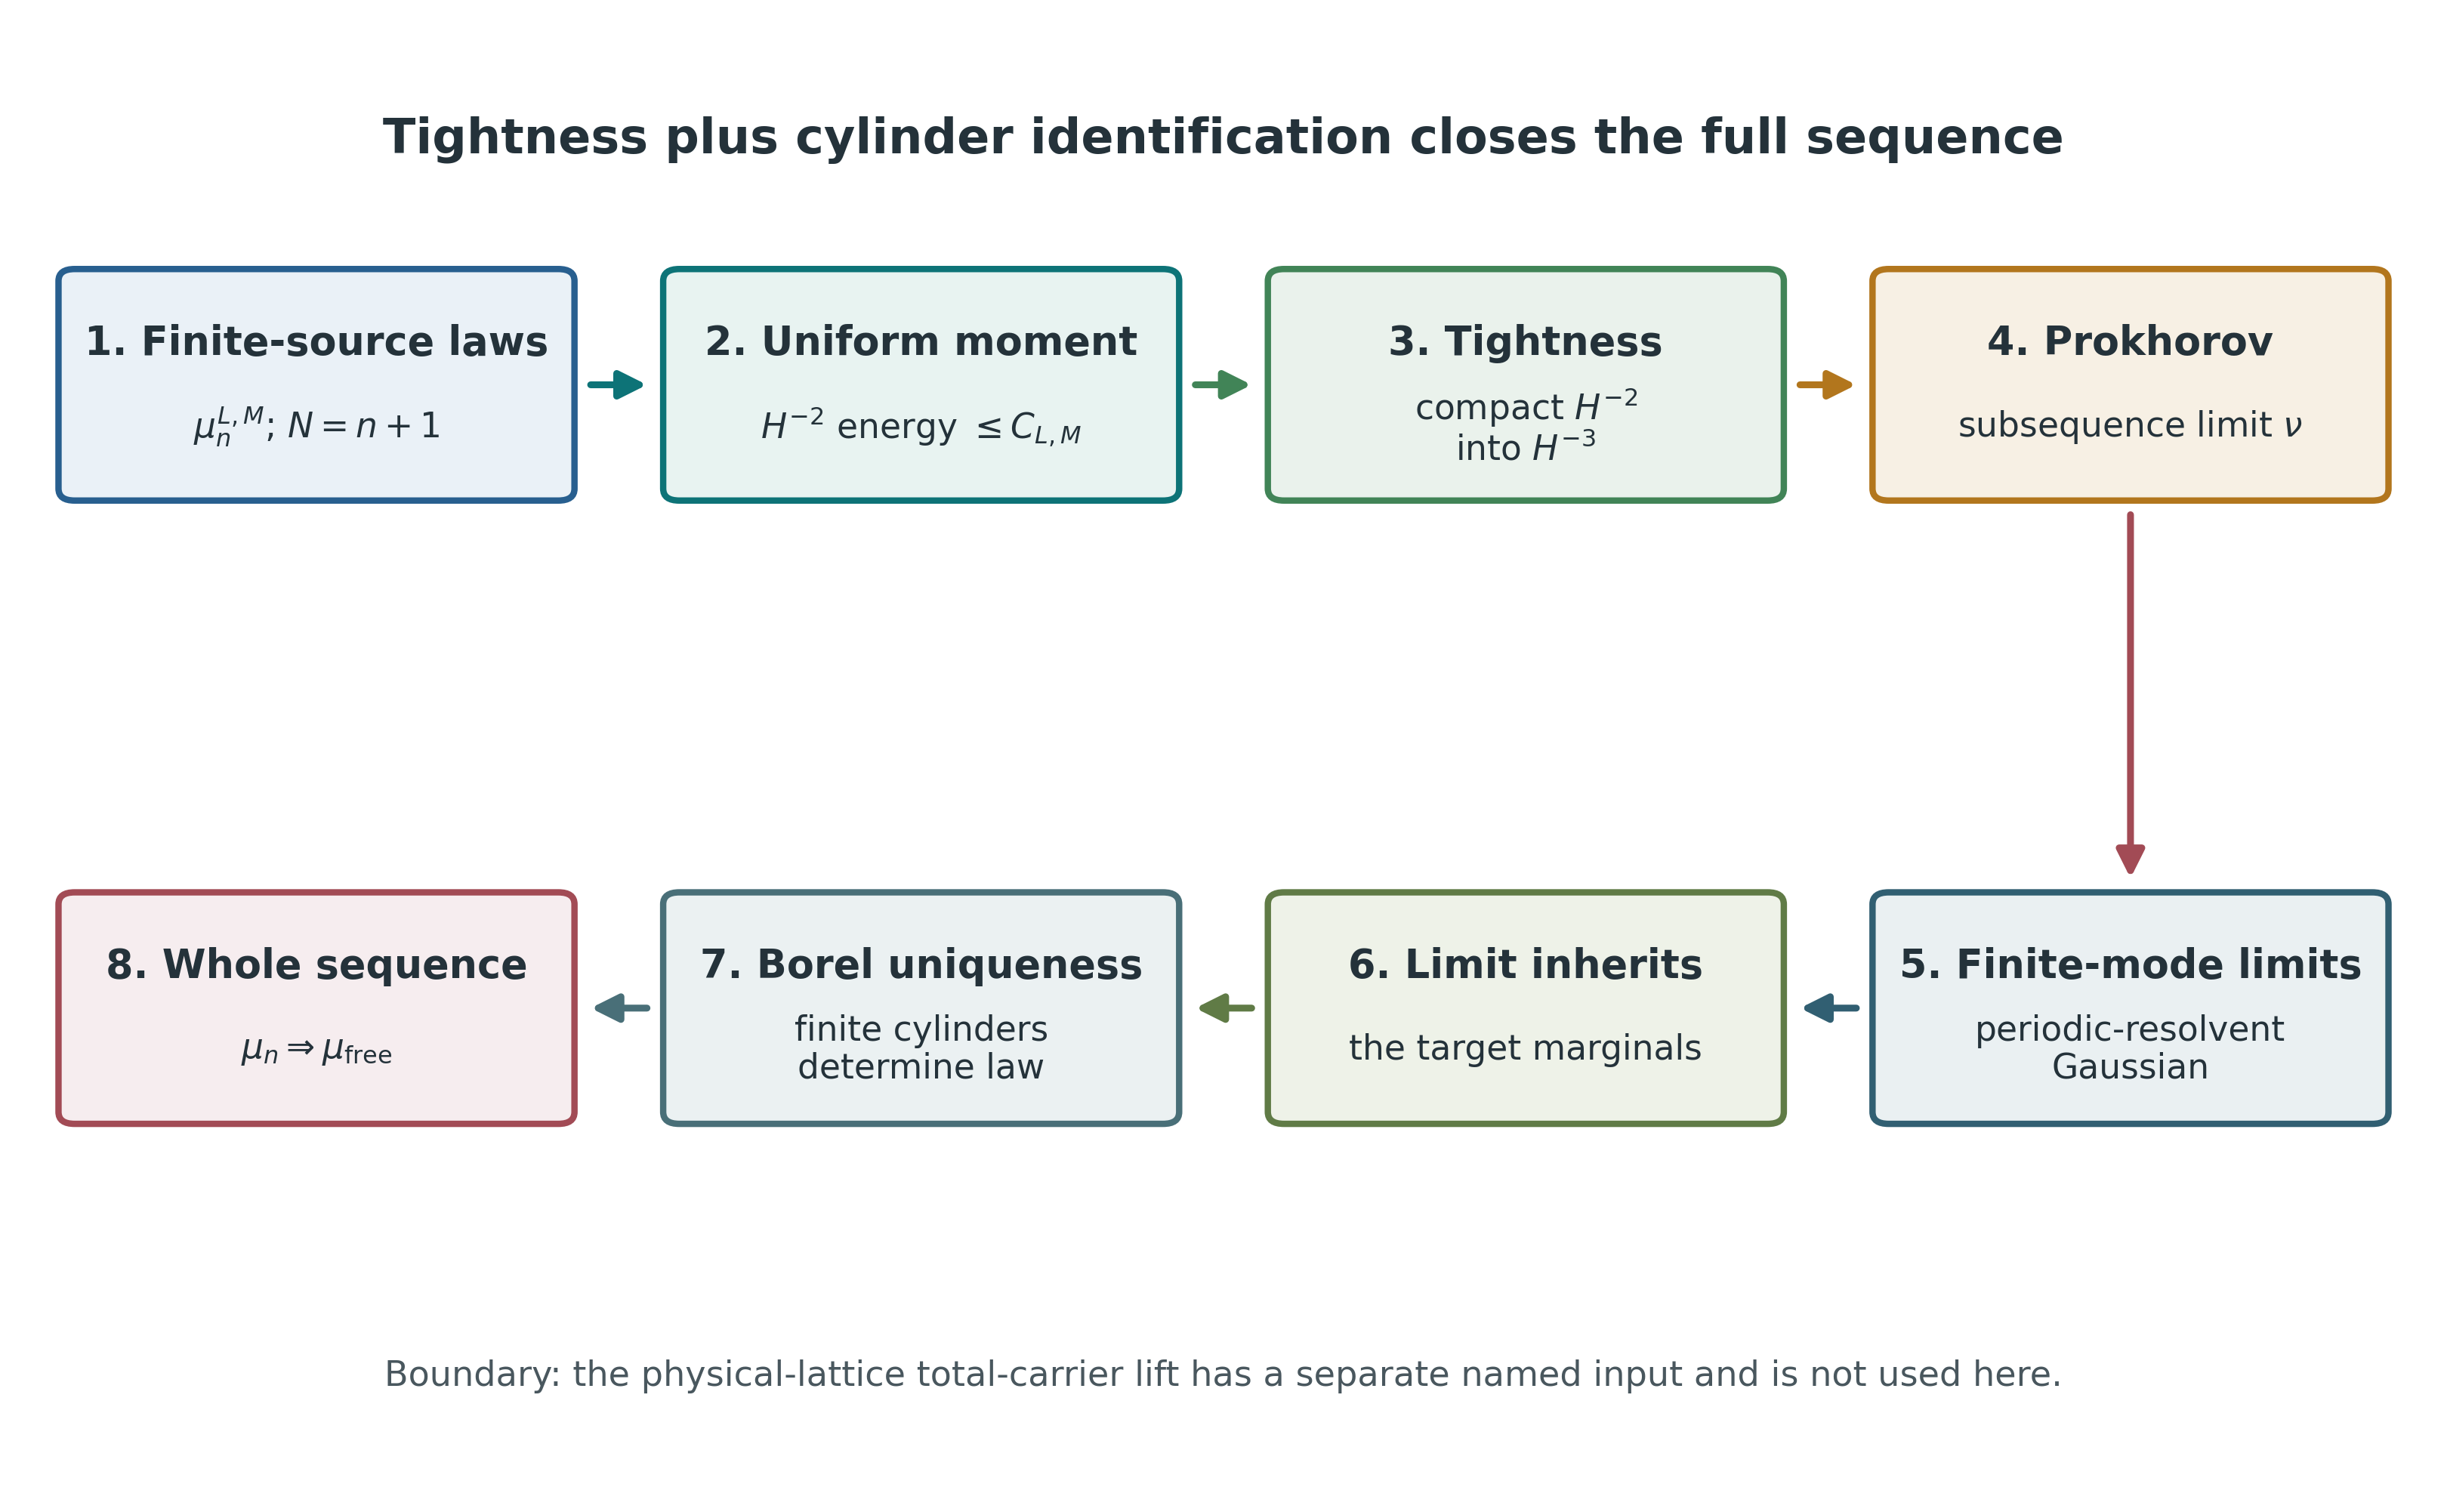
\includegraphics[width=0.98\linewidth]{figures/weak_limit_spine.png}
  \caption{Proof-dependency map for Theorem~\ref{thm:main}. Read the upper row from left to right, then continue from the upper-right box to the lower-right box and follow the lower row back toward the left: the moment bound yields tightness and subsequential limits; finite-mode convergence fixes their Gaussian marginals; Borel cylinder uniqueness identifies all limits and closes whole-sequence convergence. The displayed figure is a generated explanatory diagram, not independent mathematical evidence.}
  \label{fig:proof-spine}
\end{figure}

\appendix
\section{Formal evidence and reproducibility}
\label{app:formal-evidence}

The proof is assembled in the public Lean package \url{AImathPPhi2Clean/}, using toolchain \url{v4.34.0-rc2}. The formal development uses Lean 4 and the community mathematical library~\cite{demoura2021,mathlib2020}. The repository's \url{MANIFEST.sha256} binds the published files byte-for-byte. The principal theorem is declared in \url{AImathPPhi2Clean/PeriodicHMinusThreeWeakLimitMarginal.lean}. The following list identifies the role of each proof stage.

\begin{description}
\item[Sequence.] The construction gives the finite Gaussian pushforward. Its lattice size is $N=n+1$, with spacing $a=L/(n+1)$.
\item[Tightness.] A uniform trace bound controls the negative-order-two energy. Compact inclusion into the negative-order-three carrier and Markov's inequality yield tightness.
\item[Extraction.] The carrier is separable and complete; Prokhorov's theorem gives a Borel subsequential limit.
\item[Marginals.] Covariance convergence identifies each finite weighted Fourier marginal with the periodic-resolvent Gaussian, including degenerate cases.
\item[Uniqueness.] Finite-coordinate cylinders generate the carrier Borel sigma-algebra. Thus the marginals determine the measure.
\item[Conclusion.] Uniqueness makes all subsequential limits equal; hence the sequence converges, proving Theorem~\ref{thm:main}.
\end{description}

The separate total-carrier lift is not a premise of the assembled theorem: it requires a named measurability and representative-agreement input, as stated in Section~\ref{sec:scope}.

Figure~\ref{fig:proof-spine} was rendered with Matplotlib~\cite{hunter2007}. Procedural visualization guidance used during figure preparation is cited for workflow provenance only, not as evidence for any mathematical claim~\cite{kassis2026}.

\bibliographystyle{refs}
\bibliography{refs}

\end{document}
